\documentclass{beamer}

\usepackage{graphicx,helvet,textpos,times,verbatim,tikz,enumerate,url}%
\usepackage{wrapfig}
\usepackage{color}
\usepackage{extarrows,amsmath}
\usetheme{metropolis}           % Use metropolis theme

%=================================
%below for the tikz
\usepackage{amsfonts,mathrsfs,pifont,bbding,pgfpages}
\usepackage[latin1]{inputenc}%
\usepackage[normalem]{ulem}
\usepackage{MnSymbol,wasysym}

% TikZ styles for drawing
\usetikzlibrary{intersections}
\usetikzlibrary{arrows,shapes,shadows,positioning,automata,patterns}
\usetikzlibrary{trees,snakes,decorations.pathmorphing,decorations.markings}
\usetikzlibrary{shapes.geometric,backgrounds,calc}

% TikZ styles for drawing
\tikzstyle{block} = [draw,rectangle,rounded corners,thick,minimum height=2em,minimum width=2em,fill=blue!20,draw=black!40]
\tikzstyle{block0} = [draw,rectangle,rounded corners,thick,minimum height=2em,minimum width=2em,fill=white!20,draw=white!90]
\tikzstyle{blockr} = [draw,rectangle,rounded corners,thick,rounded corners=6,thick,minimum height=2em,minimum width=2em,black!90,fill=gray!30]
\tikzstyle{sum} = [draw,circle,inner sep=0mm,minimum size=5mm,thick,fill=gray!40]
\tikzstyle{connector} = [->,thick]
\tikzstyle{blockex} = [draw,rectangle,rounded corners,thick,minimum height=2em,minimum width=2em,thick,fill=gray!20]
\tikzstyle{blockexg} = [draw,rectangle,rounded corners,thick,minimum height=2em,minimum width=2em,thick,fill=gray!20]
\tikzstyle{line} = [thick]
\tikzstyle{branch} = [circle,inner sep=0pt,minimum size=1mm,fill=black,draw=black,black]
\tikzstyle{branch2} = [circle,inner sep=0pt,minimum size=1mm,fill=black,draw=black]
\tikzstyle{guide} = [thick]
\tikzstyle{snakeline} = [connector, decorate, decoration={pre length=0.2cm,
                         post length=0.2cm, snake, amplitude=.4mm,
                         segment length=2mm},thick, ->]
\tikzstyle{place}=[circle,thick,draw=black!75,fill=gray!20,minimum size=6mm]%

\renewcommand{\vec}[1]{\ensuremath{\boldsymbol{#1}}} % bold vectors
\def \myneq {\skew{-2}\not =} % \neq alone skews the dash
%\newtheorem{myLemma}{Lemma}[section]



%=============================================
\title{Applied Nonlinear Control \\
        \large Chapter 6 ~-~ Feedback Linearization}
\author{\large Shuai Qian}
\date{\today}
\institute{School of Automation \\
        Nanjing University of Science and Technology}
%insert the page number and the total number in footline
\setbeamertemplate{footline}[frame number]


\begin{document}
  \maketitle

%contents---------------------------
  \begin{frame}
  \addtocounter{framenumber}{-2}
  \frametitle{Table of Contents}
  \thispagestyle{empty}
  \tableofcontents
  \end{frame}

%===================================================
  \section{6.0  Introduction}

  \begin{frame}{Introduction}
    \textbf{\textit{Central ideal of feedback linearization}}
    \begin{itemize}
      \item {\color{red}Algebraically} transform a nonlinear system dynamics into a (fully or partly) linear one, so that linear control techniques can be applied
    \end{itemize}

    \textbf{\textit{Feedback Linearization V.S. Conventional Linearization}}
    \begin{itemize}
      \item \textcolor{red}{Feedback linearization} : achieved by exact state transformations and feedback
      \item \textcolor{red}{Conventional linearization} (Jacobian linearization) : linear approximations of the dynamics
    \end{itemize}
   \end{frame}


   \begin{frame}{Jacobian Linearization}
    Consider a nonlinear autonomous system
    \begin{equation}\label{nonlinear}
      \dot{\vec{x}} = \vec{f(x)}
    \end{equation}
    Assume $\vec{f(x)}$ is continuously differentiable, then
    $$
    \dot{\vec{x}} = (\frac{\partial \vec{f}}{\partial \vec{x}})_{\vec{x}=0} + \vec{f}_{h.o.t.}(\vec{x})
    $$
    (0 is an equilibrium point, $\vec{f}(0) = 0$).
    Let $\vec{A}$ denotes the Jacobian matrix of $\vec{f}$ with respect to $\vec{x}$ at $\vec{x}=0$
    $$
    {\color{red}\vec{A} = (\frac{\partial \vec{f}}{\partial \vec{x}})_{\vec{x}=0}}
    $$
    Then, the system
    $$
    {\color{red}\dot{\vec{x}} = \vec{Ax}}
    $$
   \end{frame}


%========================================================
  \section{6.1 Intuitive Concepts}

  \begin{frame}{Example}
    Consider the control of the level $h$ of fluid in a tank (Figure \ref{tank}) to a specified level $h_{d}$.
    %place the figure and word together!
    \begin{wrapfigure}{l}{4cm}
    \vspace{-10pt}
    \includegraphics[width=4cm]{image/tank.pdf}\\
    \vspace{-15pt}
    \caption{Fluid level control in a tank}\label{tank}
    \vspace{-10pt}
    \end{wrapfigure}
    Variables:
    \begin{itemize}
      \item \small{Control input} : $u$
      \item \small{Cross section of the tank} : $A(h)$
      \item \small{Cross section of the outlet pipe} : $a$
      \item \small{Desired level} : $h_{d}$
    \end{itemize}
    The dynamic model of the tank is
    \begin{equation}\label{dynamic}
      {\color{red}\frac{d}{dt}\left[\int_{0}^{h}A(h)dh\right] = u(t) - a \sqrt{2gh}}
    \end{equation}
  \end{frame}


  \begin{frame}{Feedback Linearization}
  The dynamic (\ref{dynamic}) can be rewritten as
  $$ A(h)\dot{h} = u-a\sqrt{2gh} $$
  If we choose $u(t)$ as
  $$
  Origin~dynamic \quad \xrightarrow[linearization]{{\color{red} u(t) = a\sqrt{2gh} + A(h)v}} \quad \dot{h}=v
  $$
  \vspace{-20pt}
  \begin{itemize}
    \item $v$ : \textbf{``equivalent input"} to be specified. Choosing as
  \end{itemize}
  $$
   \dot{h}=v \quad \xrightarrow[close-loop]{{\color{red} v=-\alpha \widetilde{h}}} \quad \dot{h}+\alpha \widetilde{h}=0
  $$
  \vspace{-20pt}
  \begin{itemize}
    \item $\widetilde{h} = h(t)-h_{d}$, \textbf{level error}, $\widetilde{h}(t)\rightarrow 0 ~\text{as}~ t \rightarrow \infty$
    \item $\alpha$, strictly positive constant
  \end{itemize}
  \end{frame}


  \begin{frame}{Feedback Linearization, ctd'}
  Finally, the actual input flow is
  $$ u(t) = a\sqrt{2gh} - A(h)\alpha \widetilde{h} $$ 
    The idea of \textbf{canceling the nonlinearities} and \textbf{imposing a desired linear dynamics}, can be applied to {\color{red}companion form, or controllability canonical form}:
    \begin{equation}\label{companion}
      x^{(n)} = f(\textbf{x}) + b(\textbf{x})u
    \end{equation}
    \vspace{-20pt}
    \begin{itemize}
      \item $u$ : scalar control input
      \item $x$ : scalar output of interest
      \item $\textbf{x} = \left[ x,\dot{x},\dots,x^{(n-1)}\right]^{T}$ : state vector
      \item $f(\textbf{x}), b(\textbf{x})$ : nonlinear functions of the states
    \end{itemize}
  \end{frame}


  \begin{frame}{Feedback Linearization, ctd'}
  In state-space representation, (\ref{companion}) can be written
  $$
  \frac{d}{dt}\left[\begin{array}{c}
                      x_{1} \\
                      \dots \\
                      x_{n-1} \\
                      x_{n}
                    \end{array}\right] = \left[\begin{array}{c}
                                                 x_{2} \\
                                                 \dots \\
                                                 x_{n} \\
                                                 f(\textbf{x}+b(\textbf{x})u)
                                               \end{array}\right]
  $$
  Using the control input ($b \neq 0$)\footnote{In our example, $b=\frac{1}{A(h)}, ~ f=-\frac{a\sqrt{2gh}}{A(h)}$}
  \begin{equation}\label{input}
    u = \frac{1}{b}\left[v-f\right]
  \end{equation}
  %(in example, $b=\frac{1}{A(h)}, ~ f=-\frac{a\sqrt{2gh}}{A(h)}$) \\
  we can cancel the nonlinearities and obtain the simple input-output relation
  $$ x^{(n)} = f(\textbf{x}) + b(\textbf{x})u \quad \xrightarrow[linearization]{E.q.(\ref{input})} \quad x^{(n)} = v $$
  \end{frame}


  \begin{frame}{Feedback Linearization, ctd'}
    Thus, the control law
    $$ {\color{red}v = -k_{0}x-k_{1}\dot{x}- \dots - k_{n-1}x^{(n-1)}} $$
    with the ${\color{red}k_{i}}$ chosen s.t. the polynomial
    $$p^{n}+k_{n-1}p^{n-1} + \dots + k_{0}=0$$ 
    has all its roots strictly in the left-half complex plane, leads to the {\color{red}exponentially stable dynamics}
    $$
    x^{n}+k_{n-1}x^{n-1}+\dots+k_{0}x = 0
    $$
    which implies that $x(t) \rightarrow 0$.
  \end{frame}


  \begin{frame}{Feedback Linearization, ctd'}
    For tracking of a desired output $x_{d}(t)$, the control law
    \begin{equation}\label{tracking}
      {\color{red}v = x_{d}^{(n)} - k_{0}e - k_{1}\dot{e}-\dots-k_{n-1}e^{(n-1)}}
    \end{equation}
    \vspace{-20pt}
    \begin{itemize}
        \item Leads to exponentially convergent tracking
        \item $e(t) = x(t)-x_{d}(t)$ : the tracking error
    \end{itemize}
    \textcolor{red}{In our example}, $x_{d}(t)=h_{d}$ is constant, so choose
    $$v=-\alpha(h(t) - h_{d})$$
    with the $\alpha > 0$ leads to the exponentially stable dynamics
    $$ \dot{x} + \alpha x=0 $$
  \end{frame}


  \begin{frame}{Input-State Linearization}
    Consider the single-input nonlinear system
    $$ \dot{x} = f(x,u) $$
    The technique of \textbf{input-state linearization} solves this problem in two steps :
    \begin{enumerate}
      \item Find a \textbf{state transformation} $z=z(x)$, and an \textbf{input transformation} $u=u(x,v)$ :
          $$ \dot{x} = f(x,u) \quad \xrightarrow[u=u(x,v)]{z=z(x)} \quad \underbrace{\dot{z}=Az+bv}_{{\color{red}LTI}} $$
      \item Uses standard linear techniques (such as pole placement) to design $v$.
    \end{enumerate}
  \end{frame}


  \begin{frame}{Example}
  Consider the system with the equilibrium point $(0, 0)$
  \begin{equation}\label{input-state-example}
  \begin{aligned}
    \dot{x}_{1} &= -2x_{1}+ax_{2}+\underbrace{\sin x_{1}}_{nonlinearity} \\
    \dot{x}_{2} &= \underbrace{-x_{2}\cos x_{1} + u \cos(2x_{1})}_{nonlinearity}
  \end{aligned}
  \end{equation}
  Given the new set of state variables:
  $$ {\color{red} z_{1}=x_{1} , \quad z_{2}=ax_{2} + \sin x_{1}} $$
  then, the new state equations are
    \begin{equation}\label{new-state}
      \begin{aligned}
        \dot{z}_{1} &= -2 z_{1}+z_{2} \\
        \dot{z}_{2} &= -2 z_{1} \cos z_{1}+\cos z_{1} \sin z_{1}+a u \cos \left(2 z_{1}\right)
      \end{aligned}
    \end{equation}
  \end{frame}


  \begin{frame}{Example, ctd'}
  Now, the nonlinearities can be canceled by the control law
  $$
    {\color{red}u=\frac{1}{a \cos \left(2 z_{1}\right)}\left(v-\cos z_{1} \sin z_{1}+2 z_{1} \cos z_{1}\right)}
  $$
  where $v$ is an \textbf{equivalent input} to be designed, leading to a linear input-state relation
  \begin{equation}\label{input-state-relation}
    \begin{aligned}
      \dot{z}_{1} &= -2z_{1} + z_{2} \\
      \dot{z}_{2} &= v
    \end{aligned}
  \end{equation}
  \vspace{-10pt}
\begin{figure}
  \centering
    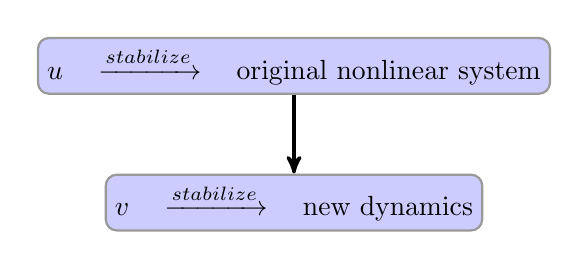
\begin{tikzpicture}[scale=0.5, auto, >=stealth']
      \matrix[ampersand replacement=\&, row sep=1cm, column sep=0.8cm]{
      \node [block] (origin) {$u \quad \xrightarrow{stabilize} \quad \text{original nonlinear system}$}; \\
      \node [block] (new) {$v \quad \xrightarrow{stabilize} \quad \text{new dynamics}$};\\
      };
      \draw [connector, very thick] ($(origin.south)$) --node{} (new);
    \end{tikzpicture}
    \end{figure}
  \end{frame}


\begin{frame}{Input-State Linearization, ctd'}
      The \textbf{closed-loop system} under the above control law is represented in the block diagram in Figure \ref{block}.
  \begin{figure}
  \centering
      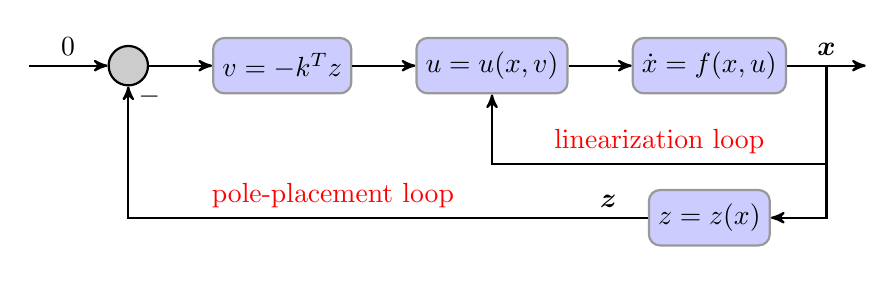
\begin{tikzpicture}[scale=0.5, auto, >=stealth']
      \matrix[ampersand replacement=\&, row sep=0.4cm, column sep=0.8cm]{

        \node[sum] (add) {};\&
        \node[block] (v) {$v=-k^{T}z$};\&
        \node[block] (u) {$u=u(x, v)$};\&
        \node[block] (dotx) {$\dot{x}=f(x,u)$}; \\
        \& \& \& \\
        \& \& \& \\
        \& \& \&
        \node[block] (z) {$z=z(x)$}; \\
        };

        %draw the lines
        \draw [connector, thick] ($(add.west)+(-2cm, 0cm)$) --node{0} ($(add.west)+(0cm, 0cm)$);
        \draw [connector, thick] ($(add.east)$) --node{} (v);
        \draw [connector, thick] ($(v.east)$) --node{} (u);
        \draw [connector, thick] ($(u.east)$) --node{} (dotx);
        \draw [connector, thick] ($(dotx.east)$) --node[above]{\vec{x}} ($(dotx.east)+(2cm, 0cm)$);
        \draw [connector, thick] ($(dotx.east)+(1cm, 0cm)$) |- ($(z.east)$);

        %for control the position of word, we can divide a line into segments!
        \draw [connector, thick] ($(z.west)$) -- node [above] {\vec{z}} ($(z.west)+(-2cm, 0cm)$) -- node [near end,above] {\textcolor{red}{ pole-placement loop}} ($(z.west)+(-10cm, 0cm)$) -| ($(add.south)+(0cm,-1cm)$) -- node [near end,right] {$-$} (add);
        \draw [connector, thick] ($(dotx.east)+(1cm, -2.5cm)$) -| node [near start,above] {\textcolor{red}{linearization loop}} (u);
      \end{tikzpicture}
  \caption{Input-State Linearization}
  \label{block}
  \end{figure}
\end{frame}


%\begin{frame}{Remarks}
%    \begin{itemize}
%      \item The result, though valid in a \textbf{large region} of the state space, is {\color{red}not global}.($x_{1}=(\pi/4 + k\pi/2), k=1,2,\dots$)
%      \item In order to implement the control law, ($z_{1}, z_{2}$) \textbf{must be available}. ~If they are not physically meaningful or cannot be measured directly, the \textbf{original state} \vec{x} must be measured and used to compute them.
%      \item In general, we rely on the system model both for the \textbf{controller design} and for the \textbf{computation of} $\textbf{z}$.
%    \end{itemize}
%\end{frame}


\begin{frame}{Input-Output Linearization}
    Consider the \textbf{tracking control problem}, and the system
    \begin{equation}\label{tracking-control}
      \begin{aligned}
        \dot{\vec{x}} &= \vec{f}(\vec{x}, u) \\
        y &= h(\vec{x})
      \end{aligned}
    \end{equation}
    \textit{\textbf{intuitive basis} for input-output linearization approach}
    \begin{enumerate}
      \item \textcolor{red}{Objective} : make the output $y(t)$ track a desired trajectory $y_{d}(t)$ while keeping the whole state bounded.
      \item \textcolor{red}{Difficulty} : output $y$ is only indirectly related to the input $u$.
      \item \textcolor{red}{Try} : if we can find a direct and simple relation between the system output $y$ and the control input $u$ ?
    \end{enumerate}
\end{frame}


\begin{frame}{Example}
Consider the third-order system:
    \begin{equation}\label{third-order}
      \left\{\begin{aligned}
        \dot{x}_{1} &= \sin x_{2}+(x_{2}+1)x_{3} \\
        \dot{x}_{2} &= x_{1}^{5}+x_{3} \\
        \dot{x}_{3} &= x_{1}^{2}+u \\
        y &= x_{1}
      \end{aligned}\right.
    \end{equation}
We find:
    $$
    \dot{y}=\dot{x}_{1}=\sin x_{2}+\left(x_{2}+1\right) x_{3}
    $$
    \begin{equation}\label{double}
      \ddot{y}=\left(x_{2}+1\right) {\color{red}u} +f_{1}(x)
    \end{equation}
where $f_{1}(x)$ is a function of the state defined by
    \begin{equation}\label{f1x}
        f_{1}(x)=\left(x_{1}^{5}+x_{3}\right)\left(x_{3}+\cos x_{2}\right)+\left(x_{2}+1\right) x_{1}^{2}
    \end{equation}
\end{frame}


\begin{frame}{Example,ctd'}
    Clearly, (\ref{double}) represents an \textbf{explicit relationship} between {\color{red}$y$} and {\color{red}$u$}.  If we choose the control input {\color{red}$u$}
    $$
         \ddot{y}=\left(x_{2}+1\right) u+f_{1}(x) \quad \xrightarrow{ {\color{red}u=\frac{1}{x_{2}+1}\left(v-f_{1}\right)}} \quad \underbrace{\ddot{y} = v}_{\tiny linear~double-integrator}
    $$
    Choosing $v$ as
    \begin{equation}\label{choose-v}
        v = \ddot{y}_{d}-k_{1}e-k_{2}\dot{e}
    \end{equation}
    where $e=y(t)-y_{d}(t)$, and $k_{1}, k_{2} > 0$. We obtain
    $$\ddot{e}+k_{2} \dot{e}+k_{1} e = 0$$
which represents an {\color{red}exponentially stable} error dynamics.
\end{frame}


\begin{frame}{Some Concepts}
    \begin{itemize}
        \item {\color{red}Relative Degree $r$}: \textbf{differentiate the output of a system $r$ times} to generate an explicit relationship between the output $y$ and input $u$
        \item {\color{red}Internal Dynamics} : a part of the system dynamics (described by one state component) has been \textbf{rendered             ``unobservable''} in the input-output linearization
        \item {\color{red}Zero-Dynamics} : the internal dynamics of the system when the system \textbf{output is kept at zero} by the input
    \end{itemize}
\end{frame}

%========================================================
\section{6.2  Mathematical Tools}


\begin{frame}{Introduction}
Every vector function \vec{f} corresponds a field of vectors in an $n$-dimensional space
$$
\text{A {\color{red}vector function}}~\vec{f}:\mathbb{R}^{n}\rightarrow \mathbb{R}^{n} \quad \xrightarrow[geometry]{differential} \quad \text{A {\color{red}vector field} in}~ \mathbb{R}^{n}
$$

\begin{itemize}
  \item given a smooth scalar function $h(\vec{x})$ of the state \vec{x}, the gradient of $h$ is denoted by $\nabla h$
      $$
      {\color{red}\nabla h = \frac{\partial h}{\partial \vec{x}}}, \quad (\nabla h)_{j} = \frac{\partial h}{\partial x_{j}}
      $$
  \item given a vector field $\vec{f}(\vec{x})$, the \textbf{Jacobian} of \vec{f} if denoted by $\nabla \vec{f}$
      $$
      {\color{red}\nabla f = \frac{\partial \vec{f}}{\partial \vec{x}}}, \quad (\nabla \vec{f})_{ij} = \frac{\partial f_{i}}{\partial x_{j}}
      $$
\end{itemize}
\end{frame}


\begin{frame}{Lie Derivatives}
    \begin{definition}[6.1]
    \textit{
        Let $h : \mathbb{R}^{n} \rightarrow \mathbb{R}$ be a smooth scalar function, and $\vec{f} : \mathbb{R}^{n} \rightarrow \mathbb{R}^{n}$ be a smooth vector field on $\mathbb{R}^{n}$, then the \underline{Lie derivative of $h$ with}
        \underline{respect to \vec{f}} is a scalar function defined by {\color{red} $L_{\vec{f}}h = \nabla h ~\vec{f}$}.
        }
    \end{definition}

    The Lie derivative $L_{\vec{f}}h$, simply : \\
    the \textbf{directional derivative} of $h$ \textbf{along the direction of the vector \vec{f}}.
    \begin{itemize}
      \item $L_{\vec{f}}^{0}h = h$
      \item $L_{\vec{f}}^{i}h = L_{\vec{f}}(L_{\vec{f}}^{i-1}h) = \nabla(L_{\vec{f}}^{i-1}h )\vec{f}$
      \item $L_{\vec{g}}L_{\vec{f}}h = \nabla(L_{\vec{f}}h)g $
    \end{itemize}
\end{frame}

\begin{frame}{Example}
    Seeing the relevance of {\color{red}Lie derivatives} to {\color{red}dynamic systems}.
    \\
    Considering the following single-output system
    $$
    \begin{array}{l}{\dot{\mathbf{x}}=\mathbf{f}(\mathbf{x})} \\ {y=h(\mathbf{x})}\end{array}
    $$
    The derivatives of the output are
    $$
    \begin{array}{l}{\dot{y}=\frac{\partial h}{\partial \vec{x}} \dot{\vec{x}}= \nabla h~\vec{f} = L_{\vec{f}} h} \\ \\
    {\ddot{y}=\frac{\partial\left[L_{\vec{f}} h\right]}{\partial \vec{x}} \dot{\vec{x}} = \nabla(L_{\vec{f}}h)\vec{f} = L_{\vec{f}}(L_{\vec{f}}h) = L_{\vec{f}}^{2} h}\end{array}
    $$
    and so on.
\end{frame}


\begin{frame}{Lie Brackets}
    \begin{definition}[6.2]
    \textit{
        Let \vec{f} and \vec{g} be two vector fields on $\mathbb{R}^{n}$. The \underline{Lie bracket of \vec{f}}
        \underline{and \vec{g}} is a third vector field defined by
        $$
        [\vec{f}, \vec{g}] = \nabla \vec{g} \vec{f} - \nabla \vec{f} \vec{g} \triangleq ad_{\vec{f}}\vec{g}\footnote{$ad$ stands for ``adjoint".}
        $$
        }
    \end{definition}
    %\vspace{-30pt}
    \begin{itemize}
      \item $ad_{\vec{f}}^{0}\vec{g} = \vec{g}$
      \item $ad_{\vec{f}}^{2}\vec{g} = [\vec{f}, [\vec{f}, \vec{g}]]$
      \item $ad_{\vec{f}}^{i}\vec{g} = [\vec{f}, ad_{\vec{f}}^{i-1}\vec{g}]$
    \end{itemize}
\end{frame}


\begin{frame}{Example}
    \begin{figure}
      \centering
      \includegraphics[width=11cm]{image/example6-7.pdf}
      %\caption{}\label{}
    \end{figure}
\end{frame}


\begin{frame}{Properties of Lie Brackets}
    \begin{lemma}[6.1]\textit{Lie brackets have the following properties}
    \begin{itemize}
      \item {\color{red}Bilinearity}:
        $$
        \begin{array}{l}{\left[\alpha_{1} f_{1}+\alpha_{2} f_{2}, g\right]=\alpha_{1}\left[f_{1}, g\right]+\alpha_{2}\left[f_{2}, g\right]} \\ {\left[f, \alpha_{1} g_{1}+\alpha_{2} g_{2}\right]=\alpha_{1}\left[f, g_{1}\right]+\alpha_{2}\left[f, g_{2}\right]}\end{array}
        $$
        where \vec{f}, $\vec{f}_{1}$, $\vec{f}_{2}$, $\vec{g}$, $\vec{g}_{1}$ and $\vec{g}_{2}$ are smooth vector fields, and $\alpha_{1}$ and $\alpha_{2}$ are constant scalars.

      \item {\color{red}Skew-commutativity} : \quad
      $[\vec{f}, \vec{g}] = -[\vec{g}, \vec{f}]$

      \item {\color{red}Jacobi identity} : \quad
      $L_{ad_{\vec{f}}\vec{g}}h = L_{\vec{f}} L_{\vec{g}} h - L_{\vec{g}} L_{\vec{f}} h$
    \end{itemize}
    \end{lemma}
\end{frame}


\begin{frame}{Diffeomorphisms And State Transformations}
    \begin{definition}[6.3]
    \textit{
        A function ~$\vec{\phi}$ : $\mathbb{R}^{n} \rightarrow \mathbb{R}^{n}$, defined in a region $\Omega$, is called a \underline{diffeomorphism} \footnote{https://en.wikipedia.org/wiki/Diffeomorphism} if it is smooth, and if its inverse $\vec{\phi} ^{-1}$ exists and is smooth.
        }
    \end{definition}

    \begin{itemize}
      \item Similar to the concept of \textbf{coordinate transformation}.
      \item Used to \textbf{transform a nonlinear system into another} system in terms of {\color{red}a new set of states}.
    \end{itemize}
    $$
    \vec{\phi}(\vec{x}) \xrightarrow[whole~space~\mathbb{R}^{n}]{region~\Omega} \text{global diffeomorphism} \xrightarrow{rare} \text{local diffeomorphism}\footnote{Finite neighborhood of a given point.}
    $$
\end{frame}


\begin{frame}{Diffeomorphisms And State Transformations, ctd'}
    Given a nonlinear function $\vec{\phi} (\vec{x})$, check \textbf{local diffeomorphism} by using the following lemma:
    \begin{lemma}[6.2]
    \textit{
        Let $\vec{\phi} (\vec{x})$ be a smooth function defined in a region $\Omega$ in $\mathbb{R}^{n}$. If the {\color{red}Jacobian matrix ~$\nabla \vec{\phi}$} is {\color{red}non-singular} at a point $\vec{x}=\vec{x}_{0}$ of $\Omega$, then $\vec{\phi}(\vec{x})$ defines a \textbf{local diffeomorphism} in a subregion of $\Omega$.
        }
    \end{lemma}
\end{frame}


\begin{frame}{Diffeomorphisms And State Transformations, ctd'}
Consider the dynamic system described by
    $$
    \begin{array}{l}{\dot{\vec{x}}=\vec{f}(\vec{x})+\vec{g}(\vec{x}) u} \\ {y=h(\vec{x})}\end{array}
    $$
    and let a new set of states be defined by ~${\color{red}\vec{z}=\phi(\vec{x})}$~,
    $$
    \dot{\mathbf{z}}=\frac{\partial \vec{\phi}}{\partial \mathbf{x}} \dot{\mathbf{x}}=\frac{\partial \vec{\phi}}{\partial \mathbf{x}}(\mathbf{f}(\mathbf{x})+\mathbf{g}(\mathbf{x}) u)
    $$
    Therefore, the new state-space representation is
    $$
    \begin{array}{l}{\dot{\vec{z}}=\vec{f}^{*}(\vec{z})+\vec{g}^{*}(\vec{z})u} \\ {y=h^{*}(\vec{z})}\end{array}
    $$
    where $\vec{x}=\vec{\phi}^{-1}(\vec{z})$ has been used, and the functions $\vec{f}^{*}$, $\vec{g}^{*}$ and $h^{*}$ are defined obviously.
\end{frame}


\begin{frame}{Example}
    \begin{figure}
      \centering
      \includegraphics[width=10cm]{image/ex6-8.pdf}
    \end{figure}
    \vspace{-10pt}
    $$
    \Omega = \{ (x_{1}, x_{2}), |x_{2}| < \frac{\pi}{2} \}
    $$
\end{frame}
\begin{frame}{Example}
    \begin{figure}
      \centering
      \includegraphics[width=10cm]{image/ex6-8.pdf}
    \end{figure}
    \vspace{-10pt}
    $$
    \Omega = \{ (x_{1}, x_{2}), |x_{2}| < \frac{\pi}{2} \}
    $$
    {\color{red}\large Question : how to calculates the $\vec{x}=\vec{\phi}^{-1}(\vec{z})$ ?}
\end{frame}


\begin{frame}{The Frobenius Theorem}
    \textit{The Frobenius theorem provides a \textbf{necessary and sufficient} condition for the \textbf{solvability} of a special class of \textbf{partial differential equations} (P.D.E.)}
    \\
    Consider the set of first-order P.D.E. with $n=3$
    \begin{equation}\label{partial-equation}
      \left\{ \begin{array}{c}
                \nabla h~\vec{f}=\frac{\partial h}{\partial x_{1}}f_{1}+\frac{\partial h}{\partial x_{2}}f_{2}+\frac{\partial h}{\partial x_{3}}f_{3}=0 \\
                \nabla h~\vec{g}=\frac{\partial h}{\partial x_{1}}g_{1}+\frac{\partial h}{\partial x_{2}}g_{2}+\frac{\partial h}{\partial x_{3}}g_{3}=0
              \end{array}\right.
    \end{equation}

    \begin{itemize}
      \item $f_{i}(x_{1},x_{2},x_{3}),~g_{i}(x_{1},x_{2},x_{3}), (i=1,2,3)$, known, scalar functions
      \item $h(x_{1},x_{2},x_{3})$, unknown
    \end{itemize}
\end{frame}


\begin{frame}{The Frobenius Theorem, ctd'}
    Clearly, this set of P.D.E. is uniquely defined by \vec{f} and \vec{g}
    $$
    \vec{f}=[f_{1}~f_{2}~f_{3}]^{T},\quad \vec{g}=[g_{1}~g_{2}~g_{3}]^{T}
    $$
    \vspace{-10pt}
    $$
    \exists ~h(x_{1},x_{2},x_{3}) \quad \xrightarrow{satisfied~E.q.(\ref{partial-equation})} \quad [\vec{f}, \vec{g}] ~is ~{\color{red}completely ~integrable}.
    $$

    {\color{red} Involutivity condition} on the vector fields $[\vec{f}, \vec{g}]$:\\
    E.q.(\ref{partial-equation}) has a solution $h(x_{1},x_{2},x_{3})$ ~iff
    $$\exists ~\alpha_{1}(x_{1},x_{2},x_{3})~,~\alpha_{2}(x_{1},x_{2},x_{3}) ~s.t.~[\vec{f},\vec{g}] = \alpha_{1}\vec{f}+\alpha_{2}\vec{g}$$

    i.e., if the Lie bracket of \vec{f} and \vec{g} can be expressed as a {\color{red}linear combination} of \vec{f} and \vec{g}.
\end{frame}


\begin{frame}{General Case of The Frobenius Theorem}
\begin{definition}[6.4]
\textit{A linearly independent set of vector fields $ \{ \vec{f}_{1}, \vec{f}_{2}, \dots, \vec{f}_{m} \} $ on $\mathbb{R}^{n}$ is said to be \underline{completely integrable}~ if, and only if, there exist {\color{red}$ n-m $} scalar functions $h_{1}(\vec{x}), h_{2}(\vec{x}), \dots , h_{n-m}(\vec{x})$ satisfying the system of partial differential equations
    \begin{equation}\label{differential-equation}
      {\color{red}\nabla h_{i}\vec{f}_{j} = 0}
    \end{equation}
    where $1 \leq i \leq n-m , 1 \leq j \leq m$, and the gradients $ \nabla h_{i} $ are linearly independent.}
\end{definition}

Recall E.q.(\ref{partial-equation}), we have the vector fields $\{ \vec{f}, \vec{g} \}$ on $\mathbb{R}^{3}$, therefore, we only need $3-2=1$ scalar function $h(\vec{x})$ satisfying it.
\end{frame}


\begin{frame}{General Case of The Frobenius Theorem, ctd'}
\begin{definition}[6.5]
    \textit{
    A linearly independent set of vector fields $ \{ \vec{f}_{1}, \vec{f}_{2}, \dots, \vec{f}_{m} \} $ is said to be \underline{involutive} if, and only if, there are scalar functions $\alpha_{ijk} : \mathbb{R}^{n} \rightarrow \mathbb{R} $, s.t.
    \vspace{-10pt}
        \begin{equation}\label{involutive-equation}
          {\color{red}[\vec{f}_{i}, \vec{f}_{j}](\vec{x}) = \sum_{k=1}^{m}\alpha_{ijk}(\vec{x})\vec{f}_{k}(\vec{x})}
        \end{equation}
    }
\end{definition}
\vspace{-20pt}
\begin{itemize}
  \item \textbf{Constant vector fields} are always involutive
  \item A set composed of a \textbf{single vector} \vec{f} is involutive. Indeed
  $$
  [\vec{f},\vec{f}] = (\nabla \vec{f})\vec{f} - (\nabla \vec{f})\vec{f} = 0
  $$
  \item From D.f.(6.5), checking involutive amounts to checking
  $$
  rank(\vec{f}_{1}(\vec{x}) \dots \vec{f}_{m}(\vec{x})) = rank(\vec{f}_{1}(\vec{x}) \dots \vec{f}_{m}(\vec{x}) ~~ [\vec{f}_{i}, \vec{f}_{j}](\vec{x})),~ \forall \vec{x},i,j.
  $$
\end{itemize}
\end{frame}


\begin{frame}{General Case of The Frobenius Theorem, ctd'}
    We can now state the Frobenius theorem formally
    \vspace{+20pt}
    \begin{theorem}[6.1 Frobenius]
    \textit{
      Let $\vec{f}_{1}, \vec{f}_{2}, \dots, \vec{f}_{m}$ be a set of linearly independent vector fields. The set is {\color{red}completely integrable} if, and only if, it is {\color{red}involutive}.
    }
\end{theorem}
\end{frame}


\begin{frame}{Example}
Consider the set of P.D.E. :
\vspace{-20pt}
    \begin{figure}
      \centering
      \includegraphics[width=11cm]{image/example6-9.pdf}
      %\caption{}\label{}
    \end{figure}
\end{frame}


%============================================================
\section{6.3  Input-State Linearization of SISO Systems}

\begin{frame}{Introduction}
Given a nonlinear system
$$
\dot{\vec{x}}=\vec{f}(\vec{x})+\vec{g}(\vec{x})w[u+\phi(\vec{x})] \quad \xrightarrow{v=w[u+\phi(\vec{x})]} \quad \underbrace{\dot{\vec{x}}=\vec{f}(\vec{x})+\vec{g}(\vec{x})u}_{\tiny linear~in~control~or ~affine}
$$
\vspace{-20pt}
\begin{itemize}
  \item \vec{f} and \vec{g} : smooth vector fields
  \item $w$ : invertible scalar function
  \item $\phi$ : arbitrary functional
  \item $u = w^{-1}(v)-\phi(\vec{x})$
\end{itemize}
Such affine system can be linearized by \textbf{state and input transformations}, we need to find such \textbf{transformations} and design \textbf{controllers} based on such feedback linearizations.
\end{frame}


\begin{frame}{Definition of Input-State Linearization}
    \begin{definition}[6.6]
    \textit{
    A single-input nonlinear system in the form $ \dot{\vec{x}} = \vec{f}(\vec{x}) + \vec{g}(\vec{x})u $, with \vec{f}(\vec{x}) and \vec{g}(\vec{x}) being smooth vector fields on $\mathbb{R}^{n}$, is said to be \underline{input-state linearizable} if there exists a {\color{red}region $\Omega$ in $\mathbb{R}^{n}$}, a {\color{red}diffeomorphism $ \phi : \Omega \rightarrow \mathbb{R}^{n} $}, and a {\color{red}nonlinear feedback control law}
    \begin{equation}\label{affine}
      u = \alpha(\vec{x})+\beta(\vec{x})v
    \end{equation}
    %change a way to show this
    such that the new state variables $\vec{z}=\phi(\vec{x})$ and the new input $v$ satisfy a linear time-invariant relation
    \begin{equation}\label{linear-relation}
      \dot{\vec{z}} = \vec{A}\vec{z}+\vec{b}v
    \end{equation}
    }
    \end{definition}
\end{frame}

\begin{frame}{Definition of Input-State Linearization, ctd'}
    \textit{Where}
    \begin{center}
    $\vec{A}=\left[\begin{matrix}
                    0 & 1 & 0 & . & . & 0 \\
                    0 & 0 & 1 & . & . & . \\
                    . & . & . & . & . & . \\
                    . & . & . & . & . & . \\
                    0 & 0 & 0 & . & . & 1 \\
                    0 & 0 & 0 & . & . & 0
                  \end{matrix}\right]$ , \quad
    $\vec{b}=\left[\begin{matrix}
                       0 \\
                       0 \\
                       . \\
                       . \\
                       0 \\
                       1
                     \end{matrix}\right]$
    \end{center}
    \begin{itemize}
      \item The new state \vec{z} is called the \textbf{linearizing state}
      \item $u = \alpha(\vec{x})+\beta(\vec{x})v$ is called the \textbf{linearizing control law}
      \item \textbf{Feedback linearization} is a {\color{red}special case} of \textbf{input-output linearization}, where the output function leads to a \textbf{relative degree $n$}
    \end{itemize}
\end{frame}


\begin{frame}{Definition of Input-State Linearization, ctd'}
    \begin{lemma}[6.3]
    \textit{
    An $n^{th}$-order nonlinear system is \textbf{input-state linearizable} if, and only if, there exists a scalar function $z_{1}(\vec{x})$ such that the system's \textbf{input-output linearization} with $z_{1}(\vec{x})$ as output function has relative degree $n$.}
    \end{lemma}

    i.e. , for the system:
    \begin{equation}\label{relation-equation}\nonumber
      \left\{\begin{aligned}
               \dot{\vec{z}} &= \vec{A}\vec{z}+\vec{b}v \\
               y &= z_{1}(\vec{x})
             \end{aligned}\right.
    \end{equation}
    we have {\color{red}$y^{(n)} = v$}.
\end{frame}


\begin{frame}{Conditions For Input-State Linearization}
    \begin{itemize}
      \item Can all nonlinear state equations in the form $ \dot{\vec{x}}=\vec{f}(\vec{x}) + \vec{g}(\vec{x})u $ be input-state linearized ?
      \item When do such linearizations exist ?
    \end{itemize}

    \begin{theorem}[6.2]
      \textit{
      The nonlinear system $ \dot{\vec{x}}=\vec{f}(\vec{x}) + \vec{g}(\vec{x})u $, with \vec{f}(\vec{x}) and \vec{g}(\vec{x}) being smooth vector fields, is {\color{red} input-state linearizable} if, and only if, there exists a region $\Omega$ such that the following conditions hold:
      \begin{itemize}
        \item the vector fields $\{ \vec{g}, ad_{\vec{f}}\vec{g}, \dots, ad_{\vec{f}}^{n-1}\vec{g} \}$ are \textbf{linearly independent} in $\Omega$
        \item the set $\{ \vec{g}, ad_{\vec{f}}\vec{g}, \dots, ad_{\vec{f}}^{n-2}\vec{g} \}$ is \textbf{involutive} in $\Omega$
      \end{itemize}
      }
    \end{theorem}
    The proof is omitted.
\end{frame}


%=====================================================
\section{6.4  Input-Output Linearization of SISO Systems}

\begin{frame}{Introduction}
    Consider single-input nonlinear systems
        \begin{equation}\label{nonlinear-system}
        \begin{array}{l}{\dot{\vec{x}}=\vec{f}(\vec{x})+\vec{g}(\vec{x}) u} \\ {y=h(\vec{x})}\end{array}
        \end{equation}
    By input-output linearization, we mean the generation of a {\color{red}linear differential relation} between the output $y$ and a new input $v$ in two steps:
    \begin{enumerate}
      \item Differentiate $y$ repeatedly until the input $u$ appears
      \item Design $u$ to cancel the nonlinearity
    \end{enumerate}
    However, in some cases, the step 2 may not be carried out, because the system's {\color{red}relative degree is undefined}.
\end{frame}


\begin{frame}{The Case of Well Defined Relative Degree}
    Assuming $\vec{x} \in \Omega_{\vec{x}} \subseteq \mathbb{R}^{n} $,
    $$
    \dot{y}=\nabla h(\vec{f}+\vec{g} u)=L_{\vec{f}} h(\vec{x})+L_{\vec{g}} h(\vec{x}) u
    $$
    {\color{red}If $L_{\vec{g}}h(\vec{x}) \ne 0$ for some $\vec{x}=\vec{x}_{0}$ in $\Omega_{\vec{x}}$}, we can design
    $$u=\frac{1}{L_{\vec{g}} h}\left(-L_{\vec{f}} h+v\right)$$

    {\color{red}If $L_{\vec{g}}h(\vec{x}) = 0$ for all \vec{x} in $\Omega_{\vec{x}}$}, we can differentiate $\dot{y}$ again
    $$
    y^{(i)}=L_{\vec{f}}^{i} h(\vec{x})+L_{\vec{g}} L_{\vec{f}}^{i-1} h(\vec{x}) u, \quad (i=2,3, \dots)
    $$
    until for some integer $r$ : $L_{\vec{g}} L_{\vec{f}}^{r-1} h(\vec{x}) \neq 0$
\end{frame}

\begin{frame}{The Case of Well Defined Relative Degree, ctd'}
    \begin{definition}[6.7]
    \textit{
    The SISO system is said to have \underline{relative degree} $r$ in a region $\Omega$ if, $\forall \vec{x} \in \Omega$
    $$
    \begin{array}{ll}{L_{\vec{g}} L_{\vec{f}}^{j} h(\vec{x})=0} & {0 \leq i<r-1} \\ {L_{\vec{g}} L_{\vec{f}}^{r-1} h(\vec{x}) \neq 0}\end{array}
    $$
    }
    \end{definition}
\end{frame}


\begin{frame}{The Case of Undefined Relative Degree}
    Sometimes, we are interested in the properties of the system about a {\color{red}specific operating point $\vec{x}_{0}$}.

    \begin{itemize}
      \item If $L_{\vec{g}} L_{\vec{f}}^{r-1} h(\vec{x}_{0}) \neq 0$, the system has relative degree $r$ {\color{red}at the point $\vec{x}_{0}$}
      \item If $L_{\vec{g}} L_{\vec{f}}^{r-1} h(\vec{x}_{0}) = 0$, but nonzero at some points \vec{x} arbitrarily close to $\vec{x}_{0}$, relative degree is then {\color{red} undefined} at $\vec{x}_{0}$
    \end{itemize}
\end{frame}

\begin{frame}{Example About The Case of Undefined Relative Degree}
    \begin{figure}
      \centering
      \includegraphics[width=10cm]{image/example6-11.pdf}
      %\caption{}\label{}
    \end{figure}
    \vspace{-20pt}
    \begin{figure}
      \centering
      \includegraphics[width=10cm]{image/example6-11-2.pdf}
      %\caption{}\label{}
    \end{figure}
\end{frame}


\begin{frame}{Normal Forms}
    When the relative degree {\color{red}$r<n$}, the nonlinear system (\ref{nonlinear-system}) can be transformed into {\color{red}normal form}. Let
    \begin{equation}\label{translate-state}
      \vec{\mu}=\left[\mu_{1}~\mu_{2}~\dots~\mu_{r}\right]^{T}=\left[y~\dot{y}~\dots~y^{r-1} \right]^{T}
    \end{equation}
    In a neighborhood $\Omega$ of a point $\vec{x}_{0}$, the normal form
    \begin{equation}\label{normal-form}
    \begin{aligned}
      \dot{\vec{\mu}} &= \left[\begin{matrix}
                                \mu_{2} \\
                                \dots \\
                                \dots \\
                                \mu_{r} \\
                                a(\vec{\mu}, \vec{\Psi})+b(\vec{\mu}, \vec{\Psi})u
                              \end{matrix}\right] \\
      \dot{\vec{\Psi}} &= \vec{w}(\vec{\mu}, \vec{\Psi})
    \end{aligned}
    \end{equation}
    with the output defined as
    \begin{equation}\label{normal-form-output}
      y=\vec{\mu}_{1}
    \end{equation}
\end{frame}


\begin{frame}{Normal Forms, ctd'}
    The normal form implies that, we should construct a {\color{red}diffeomorphism}
    \begin{equation}\label{diffeomorphism}
      \vec{\Phi}(\vec{x}) = \left[ \mu_{1}~\dots~\mu_{r}~\Psi_{1}~\dots~\Psi_{n-r} \right]^{T}
    \end{equation}

    s.t. the nonlinear system(\ref{nonlinear-system}) can indeed be \textbf{transformed into the normal form(\ref{normal-form})}.

    Hence, the \textbf{Jacobian} of $\Phi$ should be invertible \footnote{See Lemma 6.2}.

    i.e., the gradients $\nabla \mu_{i}(i=1, \dots, r)$ and $\nabla \Psi_{j}(j=1, \dots, n-r)$ are all \textbf{linearly independent}. The proof is omitted here.
\end{frame}

\begin{frame}{Normal Forms, ctd'}
    \begin{lemma}[6.5]
    \textit{
    If the relative degree of the system (\ref{nonlinear-system}) is $r$ in the region $\Omega$, then the gradients $\nabla \mu_{1}, \nabla \mu_{2}, \dots, \nabla \mu_{r}$ are linearly independent in $\Omega$.
    }
    \end{lemma}
\end{frame}

\begin{frame}{Example of The Normal Form}
    \begin{figure}
      \centering
      \includegraphics[width=10cm]{image/example6-12-1.pdf}
      %\caption{}\label{}
    \end{figure}
    \vspace{-20pt}
    \begin{figure}
      \centering
      \includegraphics[width=10cm]{image/example6-12-2.pdf}
      %\caption{}\label{}
    \end{figure}
\end{frame}

\begin{frame}{Example of The Normal Form, ctd'}
    \begin{figure}
      \centering
      \includegraphics[width=10cm]{image/example6-12-3.pdf}
      %\caption{}\label{}
    \end{figure}
\end{frame}


\begin{frame}{The Zero-Dynamics}
    \textit{{\color{red}Zero-dynamics}}, describes motion restricted to the $(n-r)$- dimensional smooth surface {\color{red}(manifold) $\vec{M}_{0}$} defined by {\color{red}$\vec{\mu}=0$}.
    \\
    For $\vec{x} \in \vec{M}_{0}, \forall~t>t_{0}$, we should have
    \begin{itemize}
      \item $\vec{x}(0) \in \vec{M}_{0}$
      \item Input $u$ s.t. $y^{(r)}(t)=0$
    \end{itemize}
    Therefore the system dynamics can be simply written in normal form as
    \begin{equation}\label{zero-normal-form}
      \begin{aligned}
        \dot{\vec{\mu}} &= 0 \\
        \dot{\vec{\Psi}}&= \vec{w}(0, \vec{\Psi})\quad ({\color{red}zero-dynamics})
      \end{aligned}
    \end{equation}
\end{frame}

\begin{frame}{Example About The Zero-Dynamics}
    \begin{figure}
      \centering
      \includegraphics[width=8cm]{image/example6-13.pdf}
      %\caption{}\label{}
    \end{figure}
\end{frame}


\begin{frame}{Minimum Phase of Nonlinear Systems}
    Linear systems whose zero-dynamics are stable are called {\color{red}minimum phase}, we extend to nonlinear systems.
    \begin{definition}[6.8]
        \textit{
        The nonlinear system (\ref{nonlinear-system}) is said to be {\color{red}asymptotically minimum phase} if its zero-dynamics is asymptotically stable.
        }
    \end{definition}
\end{frame}

\begin{frame}{Brief Summary}
    Essentially, controller designs based on {\color{red}input-output linearization} is to :
    \begin{itemize}
      \item Design a controller based on the linear input-output relation
      \item Check whether the internal dynamics is stable or not
    \end{itemize}
     Therefore, in the following, we will talk about
     \begin{enumerate}
       \item Local stabilization
       \item Global stabilization
       \item Tracking control
     \end{enumerate}
\end{frame}


\begin{frame}{Local Asymptotic Stabilization}
    Consider again the nonlinear system (\ref{nonlinear-system}) :
    \begin{equation}\label{nonlinear-system-2}\nonumber
        \begin{array}{l}{\dot{\vec{x}}=\vec{f}(\vec{x})+\vec{g}(\vec{x}) u} \\ {y=h(\vec{x})}\end{array}
    \end{equation}
    By means of input-output linearization, we have : {\color{red}$y^{(r)}=v$}

    Let \quad $v=-k_{r-1}y^{(r-1)} - \ldots -k_{1}\dot{y} - k_{0}y$

    where the $k_{i}$ are chosen such that the polynomial
    \begin{equation}\label{polynomial}
      K(p) = p^{r}+k_{r-1}p^{r-1}+\dots+k_{1}p+k_{0}
    \end{equation}
    has all its roots strictly in the {\color{red}left-half plane}. The actual control input $u$ can then be written
    \begin{equation}\label{control-input}
      u(\vec{x})=\frac{1}{L_{\vec{g}} L_{\vec{f}}^{r-1} y}\left[-L_{\vec{f}}^{r} y-k_{r-1} y^{(r-1)}-\ldots-k_{1} \dot{y}-k_{0} y\right]
    \end{equation}
\end{frame}


\begin{frame}{Local Asymptotic Stabilization, ctd'}
    We want to proof the simple {\color{red}linear pole-placement controller $v$} can provide guarantee about the stability of the overall system.
    \begin{theorem}[6.3]
      Assume that the system (\ref{nonlinear-system}) has relative degree $r$, and that its zero-dynamics is {\color{red}locally asymptotically stable}. Choose constants $k_{i}$ such that the polynomial (\ref{polynomial}) has all its roots strictly in the {\color{red}left-half plane}. Then, the control law (\ref{control-input}) yields a {\color{red}locally asymptotically stable closed-loop system}.
    \end{theorem}

    We proof it by writing the closed-loop dynamics in normal coordinates
\end{frame}

\begin{frame}{Proof}
    \begin{figure}
      \centering
      \includegraphics[width=10cm]{image/proof6-3.pdf}
      %\caption{}\label{}
    \end{figure}
\end{frame}
\begin{frame}{Proof, ctd'}
    If $A_{2}$ is \underline{asymptotically stable} (i.e., has all its eigenvalues strictly in the left-half plane), then the above linearized approximation of the whole dynamics is asymptotically stable, and therefore, using again Lyapunov's linearization theorem, the nonlinear system is locally asymptotically stable.

    \vspace{+10pt}
    If $A_{2}$ is only \underline{marginally stable}, stability of the closed loop system can still be derived by using the so-called \textbf{center-manifold theory}. \footnote{Byrnes and Isidori, 1988.}
\end{frame}


\begin{frame}{Example}
    Consider the nonlinear system
    \begin{equation}\label{example6-14}
      \begin{aligned}
        \dot{x}_{1} &= x_{1}^{2} x_{2} \\
        \dot{x}_{2} &= 3 x_{2}+u
      \end{aligned}
    \end{equation}
    The system's linearization at $\vec{x} = 0$ (where \vec{x}=$\left[x_{1}~x_{2}\right]^{T}$ ) is
    \begin{equation}\nonumber
      \begin{aligned}
        \dot{x}_{1} &= 0 \\
        \dot{x}_{2} &= 3 x_{2}+u
      \end{aligned}
    \end{equation}
    and thus has an {\color{red}uncontrollable mode} corresponding to a pure integrator($\dot{y}=v$).\\
    Let us define the output function
    \begin{equation}
      y=-2x_{1}-x_{2}
    \end{equation}
\end{frame}

\begin{frame}{Example, ctd'}
    Corresponding to this output, the relative degree of the system is 1, because
    $$
    \frac{d y}{d t}=-2 \dot{x}_{1}-\dot{x}_{2}=-2 x_{1}^{2} x_{2}-3 x_{2}-u
    $$
    By setting $y=0$, the associated zero-dynamics
    $$ {\color{red}\dot{x}_{1} = -2x_{1}^{3}} \quad (x_{2}=-2x_{1}~substitute~into~ \dot{x}=x_{1}^{2}x_{2})$$
    and thus is asymptotically stable. Therefore, according to Theorem 6.3, the
    control law
    $$ u=-2 x_{1}^{2} x_{2}-4 x_{2}-2 x_{1} $$
    \vspace{-10pt}
    locally stabilizes the nonlinear system \footnote{Where $v=-y$}.
\end{frame}


\begin{frame}{Global Asymptotic Stabilization}
    The approach to \textbf{global asymptotic stabilization} based on partial feedback linearization
    \begin{itemize}
      \item Consider the control problem as a {\color{red}standard Lyapunov controller design problem}
      \item Basic idea : in normal form, view {\color{red}\vec{\mu} as the ``input'' to the internal dynamics, and \vec{\Psi} as its ``output''}
    \end{itemize}
\end{frame}

\begin{frame}{Global Asymptotic Stabilization, ctd'}
    Two steps to realize this approach:
    \begin{enumerate}
      \item Find a \textbf{``control law''} $\vec{\mu}_{0}=\vec{\mu}_{0}(\Psi)$ which \textbf{stabilizes the internal dynamics}, and an associated Lyapunov function $V_{0}$ demonstrating that stabilizing property
      \item Get back to the original global control problem, define a Lyapunov function candidate {\color{red}$V$} \footnote{Appropriately as a modified version of $V_{0}$.} , and choose the {\color{red}control input $v$} so that $V$ be a Lyapunov function for the whole closed-loop dynamics
    \end{enumerate}
\end{frame}


\begin{frame}{Tracking Control}
    Consider the nonlinear system(\ref{nonlinear-system}), the problem of tracking a given desired trajectory $y_{d}(t)$. Let
    $$ \vec{\mu}_{d} = \left[ y_{d}~~\dot{y}_{d}~~y_{d}^{(r-1)} \right]^{T} $$
    and define the tracking error vector by
    $$ \widetilde{\vec{\mu}}(t)=\vec{\mu}(t) - \vec{\mu}_{d}(t) $$

    We then have the following result:
\end{frame}

\begin{frame}{Tracking Control, ctd'}
    \begin{theorem}[6.4]
      Assume that the system (\ref{nonlinear-system}) has relative degree $r$ (defined and constant over the region of interest), that $\vec{\mu}_{d}$ is smooth and bounded, and that the solution $\vec{\Psi}_{d}$ of the equation
      $$
        \dot{\vec{\Psi}}_{d}=\vec{w}\left(\vec{\mu}_{d}, \vec{\Psi}_{d}\right) \quad \vec{\Psi}_{d}(0)=\vec{0}
      $$
      exists, is bounded, and is uniformly asymptotically stable. Choose constants $k_{i}$ such that the polynomial (\ref{polynomial}) has all its roots strictly in the left-half plane. Then, by using the control law
      \begin{equation}
        {\color{red} u=\frac{1}{L_{\vec{g}} L_{\vec{f}}^{r-1} \mu_{1}}\left\{-L_{\vec{f}}^{r} \mu_{1}+y_{d}^{(r)}-k_{r-1} \widetilde{\mu}_{r}-\ldots-k_{0} \widetilde{\mu}_{1}\right\} }
      \end{equation}
      the \textbf{whole state remains bounded} and the \textbf{tracking error ~ $\widetilde{\vec{\mu}}$~ converges to zero exponentially}.
    \end{theorem}
\end{frame}

% \begin{itemize}
%  \item Tracking control to be exact from time $t = 0$ on
%  \item $\vec{\mu}(0) = \vec{\mu}_{d}(0)$
% \end{itemize}
\begin{frame}{Inverse Dynamics}
    For {\color{red}tracking a reference output $y_{r}(t)$ perfectly},
    \begin{equation}\label{thought-inverse}\nonumber
     Assume ~y(t)\equiv y_{r}(t), ~\forall t \geq 0 \quad \xrightarrow{determine}\quad \left\{
      \begin{matrix}
        \text{Initial conditions}~{\color{red}\vec{x}(0)} \\
        \text{Control input}~{\color{red}u}
      \end{matrix}\right.
    \end{equation}
    Let
    $$
    \vec{\mu}(t)=\vec{\mu}_{r}(t)=\left[\begin{array}{ll}{y_{r}(t)} & {\dot{y}_{r}(t) \ldots y_{r}^{(r-1)}(t)}\end{array}\right]^{T} , \quad \forall t \geq 0
    $$
    Thus, the control input $u(t)$ must satisfy
    $$
    {\color{red}y_{r}^{(r)}(t)=a\left(\vec{\mu}_{r}, \vec{\Psi}\right)+b\left(\vec{\mu}_{r}, \vec{\Psi} \right) u(t)}
    $$
\end{frame}

\begin{frame}{Inverse Dynamics, ctd'}
    That is, 
    \begin{equation}\label{inverse-dynamics}
      \left. \begin{aligned}
        u(t) &= \frac{y_{r}^{(r)}-a(\vec{\mu}_{r}, \vec{\Psi})}{b(\vec{\mu}_{r}, \vec{\Psi})} \\
        \dot{\vec{\Psi}}(t) &= \vec{w}\left[ \vec{\mu}_{r}(t),\vec{\Psi}(t) \right]
      \end{aligned} \right\} \quad {\color{red}inverse ~dynamics}
    \end{equation}
    \begin{itemize}
      \item Formally, $\vec{\Psi}$ is the state of the inverse dynamics, $\vec{\mu}_{r}$ its input, and $u$ its output.
    \end{itemize}
\end{frame}


\begin{frame}{Tracking Control For Non-minimum Phase System}
    \textit{\color{red}\large{Output-redefinition method}}
    \begin{itemize}
      \item The principle is to \textbf{redefine the output} function $y_{1}=h_{1}(x)$ so that the resulting zero-dynamics is stable
    \end{itemize}
    Consider the tracking control of the linear system
    \begin{equation}
        y=-\frac{\left(1-\frac{p}{b}\right) B_{o}(p)}{A(p)}u
    \end{equation}
    \begin{itemize}
      \item $b$ is a strictly positive constant
      \item The zeros of $B_{o}(p)$ are all in the left-half plane
      \item $p$ is the Laplace variable
    \end{itemize}
\end{frame}

\begin{frame}{Tracking Control For Non-minimum Phase System, ctd'}
    Define the {\color{red}``nominal output'' $y_{1}$}
    \begin{equation}\label{y1}
      y_{1}=\frac{B_{o}(p)}{A(p)}u
    \end{equation}
    $y_{d}(t)$ is desired output, and based on Theorem 6.4, one can find a control input $u$ that achieves {\color{red}convergent tracking of $y_{1}$}.
    \begin{equation}
        y(t)=\left(1-\frac{p}{b}\right) y_{1}=\left(1-\frac{p}{b}\right) y_{d}
    \end{equation}
    therefore, we have
    $$
        error = y(t)-y_{d}(t)=-\frac{\dot{y}_{d}(t)}{b}
    $$
    In particular,the error is {\color{red}bounded} as long as $\dot{y}_{d}$ is bounded.
\end{frame}
%=====================================================
%\section{6.5  *Multi-Input Systems}

%=====================================================
\section{6.5  Summary}

\begin{frame}{Summary}
    $$
    \underbrace{Nonlinear~~dynamics \quad \xrightarrow{state~feedback} \quad linear~form }_{\color{red}\large{Feedback ~Linearization}}
    $$
    \begin{itemize}
      \item {\color{red}Input-state linearization} : complete linearization
      \item {\color{red}Input-output linearization} : partial linearization
    \end{itemize}
    
    \textit{\textbf{Some important limitations}}
    \begin{enumerate}
      \item Cannot be used for all nonlinear systems
      \item Full state has to be measured
      \item No robustness is guaranteed in the presence of parameter uncertainty or unmodeled dynamics
    \end{enumerate}
\end{frame}

\begin{frame}[c]
       \centering
       \textbf{\Large Thank You for the attention !}
    
    \vspace{+30pt}
    \centering
       {\footnotesize Suggestions for providing additional services/informations are most welcome}
\end{frame}

\end{document}










